\documentclass[a4paper]{article}    %设置页面为A4
\usepackage[UTF8]{ctex}             %中文包
\usepackage[german]{babel}          %德语包
\usepackage{amsmath}                %数学计算包
\usepackage{lmodern}
\usepackage{graphicx}               %插入图片的宏包
\usepackage[margin=1in]{geometry}   %设置页边距
\usepackage{listings}               %插入代码的包
\usepackage{xcolor}                 %插入代码的包附加颜色包
\lstset{
    language=python,  %代码语言使用的是matlab
    frame=tlrb, %把代码用带有阴影的框圈起来
    rulesepcolor=\color{red!20!green!20!blue!20},%代码块边框为淡青色
    keywordstyle=\color{blue!90}\bfseries, %代码关键字的颜色为蓝色,粗体
    commentstyle=\color{red!10!green!70}\textit,    % 设置代码注释的颜色
    showstringspaces=false,%不显示代码字符串中间的空格标记
    numbers=left, % 显示行号
    numberstyle=\tiny,    % 行号字体
    stringstyle=\ttfamily, % 代码字符串的特殊格式
    breaklines=true, %对过长的代码自动换行
    extendedchars=false,  %解决代码跨页时,章节标题,页眉等汉字不显示的问题
%   escapebegin=\begin{CJK*},escapeend=\end{CJK*},      % 代码中出现中文必须加上,否则报错
    texcl=true
}

\begin{document}

\section{二分法binärer Suche、有向图、邻接表}

\subsection{binärer Suche} 

\noindent Die Zahlen 3,6,7,10,15,16,17,23,42,43,45,54,76,77,100

(a) 用二分查找,指出16是这些数字中的第六个最小的数字。

(b)	说明为什么二进制搜索只能在有序列表上使用。

(c)	解释为什么二进制搜索具有对数运行时间。

\noindent Ans:

(a) 计算从中间开始,总计15个数字,比较顺序为:23,10,16。其中,16的下标为5。
代码为:

\begin{lstlisting}
data_list = [3,6,7,10,15,16,17,23,42,43,45,54,76,77,100]
def bi_search(data_list, val):
    low = 0
    high = len(data_list) - 1
    while low<=high:
        mid = (low + high)//2
        print(data_list[mid])
        if data_list[mid] == val:
            return mid
        elif data_list[mid] > val:
            high = mid - 1
        elif data_list[mid] < val:
            low = mid + 1
    return None
ans = bi_search(data_list, 16)
print(ans)
\end{lstlisting}

(b) Sonst möglicherweise falsches Ergebnis. (Aber in log-Zeit)

(c) Jeder Schritt halbiert das Feld => O(log(n)) - viele Schritte

Jeder Schritt O(1) Zeit => insgesamt O(log(n)) Zeit.


\noindent\textbf{补充:时间复杂度计算}

O(1): 不论代码多少,只要没有循环等复杂结构,就是这个。

O(n): 1个for循环。这种代码会重复执行n次,因此说,它的时间消耗是随着n的变化而变化的。

O(log(n)): while循环。用于和n进行比较的变量为v,如果每次循环中,
v都是$\times 2$的(或者n是$\div 2$的),那么循环x次后,v就n不符合判断条件了。
也就是说,$2^x = n$,即$x = log2^n$。在这种情况下,都认为时间复杂度为O(log(n))。

O(nlog(n)): for循环中套了一个O(log(n))的循环,即,执行了n次的O(log(n))。

O($n^2$): 1个for循环嵌套1个同样需要运行n次的for循环。需要注意的是,此时与上述的for循环均要求其i均匀是$\pm 1$变化的。

O($n \times m$): 即在1个for循环嵌套1个需要运行m次的for循环。

O($n^k$): 即类似多层循环。

\subsection{有向图、邻接表} 

\noindent 有向图gerichteter Graph G 如下:

\begin{center}
    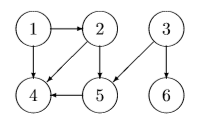
\includegraphics[scale=0.6]{1.png}
\end{center}

(a)	用邻接表表示G。

\begin{center}
    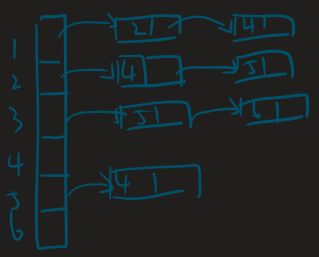
\includegraphics[scale=0.6]{2.png}
\end{center}

(b)	使用讲座中的算法,证明G是kreisfrei的,并指出每个要删除的节点。

Idee: Löschen Sie alle Knoten ohne eingehende Kanten und löschen Sie dann alle angrenzenden ausgehenden Kanten.
删除所有没有入边的节点,然后删除所有相邻的出边。

Löschung {1, 3}, Löschung {2, 6}, Löschung {5}, Löschung {4}

Wenn keine Knoten übrig sind, handelt es sich um Kreisfreis.
如果没有剩余节点,则说明是kreisfrei的。

(c)	指定节点的拓扑排序。

{1,3,2,6,5,4}

\noindent\textbf{补充:拓扑排序}

对于一个有向无环图DAG进行拓扑排序,计算规律同(b)。若kreisfrei,则输出的序列为拓扑序列。



\section{有向图、BFS、拓扑排序}

\subsection{有向图、BFS}

\noindent 有向图$G=(V,E))$,用邻接表表示。判断以下内容是否正确。
其中,不同的颜色分别对应:

weiß - u noch nicht entdeckt

grau - u entdeckt, aber noch nicht abgeschlossen, d.h. u in Schlange

schwarz - u entdeckt und abgearbeitet.


(a) 有边Kante(u,v)$\in E$,因此:Bei der Expansion von u während BFS(G,s) ist v – je nach Adjazenzlistendarstellung von G – grau oder schwarz.

\begin{center}
    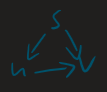
\includegraphics[scale=0.6]{3.png}
\end{center}

i. s $\rightarrow$ v,u; u $\rightarrow$ v; v 

\indent\indent s $\rightarrow$ grau; v,u werden in die Schlange eindeutigt, $\rightarrow$ grau.

\indent\indent s $\rightarrow$ schwarz, v $\rightarrow$ schwarz. $\rightarrow$ v ist bei der Expansion von u schwarz.

ii. s $\rightarrow$ u,v; u $\rightarrow$ v; v

\indent\indent s $\rightarrow$ grau; u,v werden in die Schlange eindeutigt, $\rightarrow$ grau.

\indent\indent s $\rightarrow$ schwarz. v ist bei der Expansion von u grau.


(b) 有边Kante(u,v)$\in E$,因此:Bei der Expansion von u während BFS(G,s) ist v – je nach Adjazenzlistendarstellung von G – weiß oder grau.

\begin{center}
    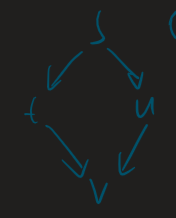
\includegraphics[scale=0.6]{4.png}
\end{center}

i. s $\rightarrow$ u $\rightarrow$ t; u $\rightarrow$ v; t $\rightarrow$ v; v

\indent\indent v ist bei der Expansion von u weiß

ii. s $\rightarrow$ t $\rightarrow$ u; t $\rightarrow$ v; u $\rightarrow$ v; v

\indent\indent v ist bei der Expansion von u grau


(c) 有边Kante(u,v)$\in E$,因此:Bei der Expansion von u während BFS(G,s) ist v – je nach Adjazenzlistendarstellung von G – weiß oder schwarz.

nicht möglich

\subsection{子树与BFS搜索树}

有向图G内含一颗树B,根为s。存在条件:$Dist_B(s,v) = Dist_G(s,v)$,即最短路径相同。然而,B树不可能是G的BFS搜索树。为什么?

\begin{center}
    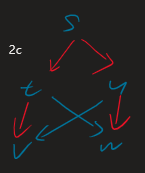
\includegraphics[scale=0.6]{5.png}
    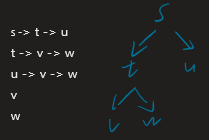
\includegraphics[scale=0.6]{6.png}
\end{center}

Ans: Die rote Kanten bilden(如左图), unabhängig von der Adj.Listendast., keinen BFS-Baum.(搜索树如右图)


\subsection{拓扑排序}

\subsubsection{} 有n个节点的序列$(v_1,...,v_n)$,有多少有向图$G=(V,E)$与节点$V=\{v_1,...,v_n\}$将此序列作为拓扑排序?

\begin{center}
    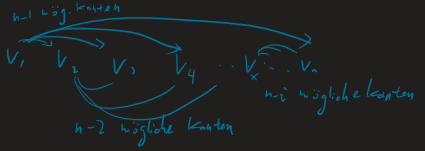
\includegraphics[scale=0.6]{7.png}
\end{center}

$\Rightarrow$总计
$\sum^n_{i=1}(n-i) = \sum^{n-1}_{i=0}=\frac{(n-1)n}{2}=\begin{pmatrix}n\\2 \end{pmatrix}$。
也就是说,Mögliche Kanten $\Rightarrow 2^{\begin{pmatrix}n\\2 \end{pmatrix}}$ Graphen

在无向图中有$\begin{pmatrix}n\\2 \end{pmatrix}$个可能的边,即有2个可能的无向图与n个给定的节点。

Wir können in einem ungerichtetem Graphen G Richtungen festlegen, sodass der gerichtete Graph einer gegebenen topologische Sortierung entspricht:
我们可以在无向图G中定义方向,以便有向图对应于给定的拓扑排序:T: topologische Sortierung


\begin{equation}
    \{u,v\}\, in\, E \Rightarrow \left\{
        \begin{array}{lr}
            T(u) < T(v) \Rightarrow (u,v)\, in\, E'\\
            T(u) > T(v) \Rightarrow (v,u)\, in\, E'
        \end{array}
    \right.
\end{equation}

\section{无向图}

\subsection{3染色问题} 有作为输入的无向图G=(V,E),设计算法:

1. G' = G

2. Solange es in G' einen Knoten u mit Grad(u)$\leq 2$ gibt: Entferne u (mit all einen Kanten) aus G'
若G'中某个节点u的度小于等于2,则删除该节点及其所有相临边。

3. Falls G' leer ist: Ausgabe 'G ist 3-färbbar'
重复2之后,若G'为空,则输出'G ist 3-färbbar'

4. Sonst: Ausgabe 'Weiß nicht'
否则输出不知道。

\noindent 求:

(a) 无向图G=(V,E)如下,求G'在每次运行中的Schritt 2状态。

\indent\indent $V=\{1,2,3,4,5,6,7\}$

\indent\indent $E=\{\{1,2\},\{2,3\},\{1,4\},\{4,3\},\{2,4\},\{1,5\},\{6,5\},\{7,5\},\{5,4\}\}$

\begin{center}
    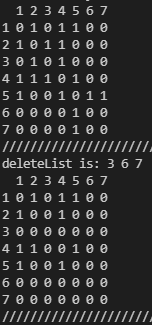
\includegraphics[scale=0.6]{8.png}
    
\includegraphics[scale=0.6]{9.png}
\end{center}

(b) 给出一个3-färbbaren G,但要运用上述算法输出"weiß nicht"。给出G'该图的(a)。

\begin{center}
    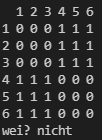
\includegraphics[scale=0.6]{10.png}
    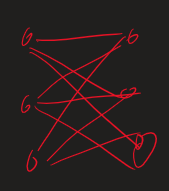
\includegraphics[scale=0.6]{11.png}
\end{center}

(c) 用数学归纳法(Induktionsbeweis)说明算法的正确性:当某个图不是3-färbbar的,则任何时候都不可能输出"G ist 3-färbbar"。

略

\subsection{2染色,bipartit,二分图} \noindent 何为二分图?

将一个图中所有的节点划分成两组,若$\forall V_i \in G. G_1,G_2 \in G$. $V_1 \in G_1, V_2 \in G_2$. 
$\forall v \in V_1, \forall u \in V_2$,
不存在边$\{v_i,v_j\}$和$\{u_i,u_j\}$。
则称此划分后的图为二分图。

代码思路是利用BFS,设置每相邻的一层节点为不同的group值。

\noindent 例:

\begin{center}
    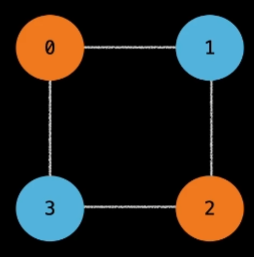
\includegraphics[scale=0.4]{12.png}
    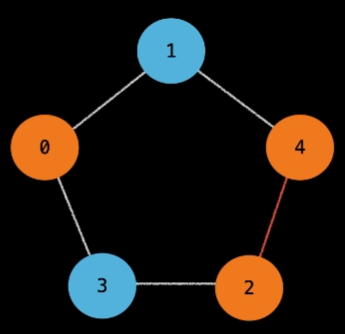
\includegraphics[scale=0.4]{13.png}
\end{center}

(上)左图可划分为二分图,右图则不能。

(下)上图的运行结果如下图。

\begin{center}
    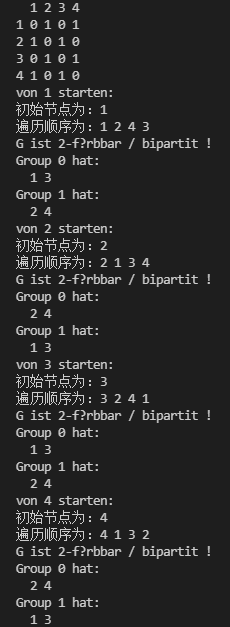
\includegraphics[scale=0.6]{14.png}
    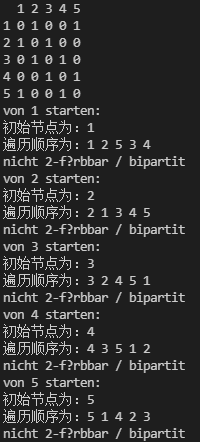
\includegraphics[scale=0.6]{15.png}
\end{center}

\section{DFS}

\subsection{Pseudocode,伪码;其在RAM中的变化}

\noindent 其中函数定义:

d[1...n]: Entdeckzeit. Nicht Entfernung wie vorher. Knoten wird grau.

f[1...n]: Beendezeit. Knoten wird schwarz.

pi[1...n]: Tiefensuchwald, wobei pi[u] = v $\Leftrightarrow$ v $\rightarrow$ u im Baum. pi[u] = "Knoten, über den u entdeckt wurde".
深度搜索森林,其中 pi [u] = v $ \Leftrightarrow $ v $ \rightarrow $ u 在树中。 pi [u] = “发现 u 的节点”。

col[1...n]: aktuelle Farbe

\subsubsection{rekurtion 递归版本}

\begin{lstlisting}[language = java]
//DFS(G)
/*1. Initialisiere 初始化*/
foreach u in V do
    col[u] = weiß;
    pi[u]=nil;
end
time = 0;

/*2. Hauptschleife 主循环:*/
foreach u in V do
    /*Aufruf von DFS-visit nur, wenn col[u] = weiß*/
    if col[u] == weiß then
        DFS-visit(u);
    end
end
\end{lstlisting}

\begin{lstlisting}[language = java]
//DFS-visit(u)
col[u] = grau;      /*Damit ist u entdeckt*/
d[u] = time;
time = time + 1;
foreach v in Adj[u] do  /*u wird bearbeitet*/
    if col[v] == weiß then  /*(u,v) untersucht*/
        pi[v] = u;      /*v entdeckt*/
        DFS-visit(v);
    end
end
/*Die Bearbeitung von u ist hier zu Ende. Sind alle Knoten aus Adj[u] grau oder schwarz, so wird u direkt schwarz.*/
col[u] = schwarz;
f[u] = time;
    /*Zeitzähler geht hoch bei Entdecken und Beenden*/
time = time + 1;
\end{lstlisting}

\subsubsection{rekurtionsfrei 无递归版本}

Idee: Gierig: Jeder weiße Knoten kommt auf dem Stack.
想法:贪心:每个白结都在堆栈上

Der Algorithmus verhält sich wie die normale Tiefensuche mit ungedreten Adjazenzlisten.
该算法的行为类似于普通的深度优先搜索,带有未修饰的邻接列表。

\begin{lstlisting}[language=java]
TS(v)
	S=stack
	S.push(v)
	while S != empty Stack
		u:=S.peek()                 //u:=S.pop(), S.push(u)
		if col(u) != weiß
		then if col(u) == schwarz then S.pop(); return;
			else 
				S.pop()
				if (u) = zeit
					zeit ++
					col(v) = schwarz
					return
		col(u) = grau
		d(u) = zeit
		zeit++
		
		for each w im AdjListe von u:
			if col(w) == weiß
			then pi(w) = u
S.push(w)
\end{lstlisting}

\noindent Brauchen wir den Stack?

ans: Nein.

	Wir finden einen weißen Kindknoten über die Adjanzliste und das col-Array.
    我们通过邻接表和 col 数组找到一个白色的子节点。

	Die Elternknoten liegen in dem pi-Array. 
    父节点在 pi 数组中。

\subsection{时间先后判断,RAM}

\noindent 存在有向图如下

\begin{center}
    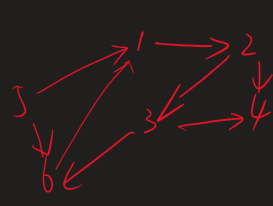
\includegraphics[scale=0.6]{16.png}
    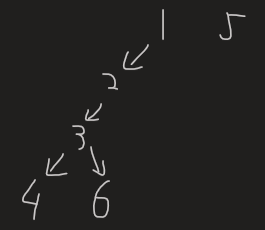
\includegraphics[scale=0.6]{17.png}
\end{center}

按照从小到大的遍历顺序,进行DFS,则遍历序列为:$1\rightarrow2\rightarrow3\rightarrow4\rightarrow6\rightarrow5$,生成树如上右图

该图证明了,即使存在例如路径\{6,5\},且6先于5被发现(即$d(6)<d(5)$),6也不是5的直接或间接前驱,5不是6的直接或间接后继。

\section{有向图的环,强连通图及其DFS拓扑排序,双连通分量,割点(桥)}

\subsection{DFS拓扑排序}

\noindent 思路:

a. 根结点入栈

b. 进行DFS,判断栈顶元素的入度是否为0,若是,则记录该点,放入待删除序列

c. DFS结束,对图进行操作,根据待删除序列,删除图中的节点和边

d. 判断是否有环:
    
\indent\indent i. 若图中存在节点的入度为0,则回到a;

\indent\indent ii. 若图中不存在入度为0的节点,且待删除序列长度不等于原始节点个数,则有环。

\indent\indent iii. 若待删除序列长度等于原始节点个数,则完全遍历完成,无环。

\indent\indent iV. 若图中不存在入度为0的节点,且待删除序列长度为0,则为强连通图。


\subsection{关节点 Artikulationspunkte}

\noindent 有无向图如下,右侧为从c开始的DFS生成树:

\begin{center}
    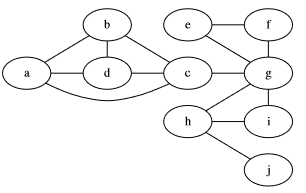
\includegraphics[scale=0.6]{18.png}
    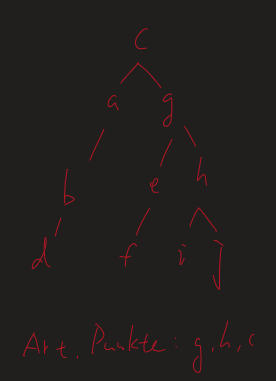
\includegraphics[scale=0.6]{19.png}
\end{center}

关节点为:g,h,c

即,删除此点与相关边后,原图会被划分成多个子图,则称此点为关节点。若原图中不存在关节点,则称此图为强连通图。

在强连通图中,至少删去k个节点,才能被分成多个子图(即破坏了图的连通性),则称该图的连通度为k。

\noindent 寻找关节点的方法如下(用DFS):

i. 根据DFS生成树,若根节点存在$\geq$2个子树,则该根节点为关节点。

ii. 若生成树中某个非叶子节点v,其某棵子树与v的全部祖先节点无连接,则v是关节点。

\subsection{连通性,tarjan算法}

\subsubsection{对于有向图}

则是寻找有向图中的强连通分量(即最大得到连通分量)。

为此,需要引入两个变量:

\indent\indent dfn[]: 时间戳。在DFS中,记录每个点第一次被访问的时间顺序。可用dfn来判断某个点是否已经遍历过。

\indent\indent low[]: 追溯值。某点x的追溯值为该点的子树中某一节点y,y拥有最小时间戳,且y满足以下条件:

\indent\indent\indent i. 该点已经访问过(有dfn值)

\indent\indent\indent ii. 存在边$(y\rightarrow z_i)$,$z_i$是x的任意祖先节点,则比较$low[z_i]$与$low[y].\,low[y]$=$min(low[z_i],low[y])$。而$low[x] = min(low[y_i],low[x])$。

在遍历时,在往回走之前,dfn[] = low[]。

其中,low[]值相同的节点存在于同一个连通子图。

\subsubsection{对于无向图}

算法类似,不过在上面的ii.中,不再要求边是$(y\rightarrow z_i)$的,而是$(y,z_i)$即可,即只要存在于$x$的任意父节点相连的边就行。

\subsubsection{例子}

有图如5.2,从c点开始,求其dfn[]和low[]值。

\begin{center}
    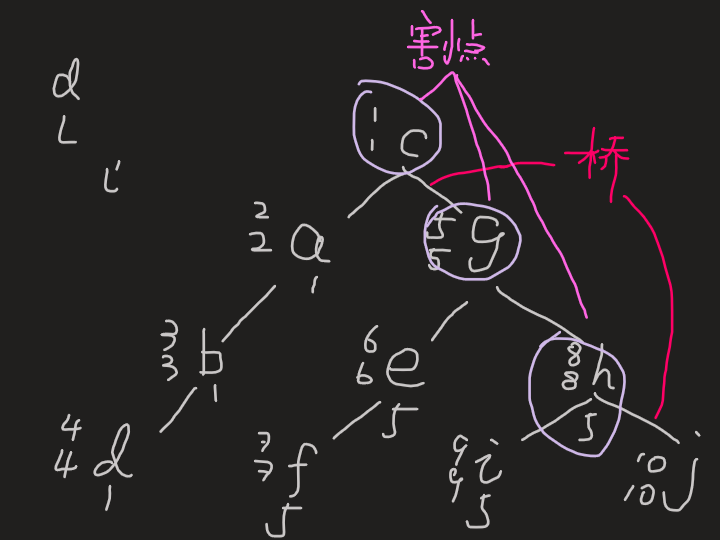
\includegraphics[scale=0.6]{46.png}
\end{center}

\subsection{双连通分量,割点(桥)}

\noindent 点双连通分量:无向图中不存在割点。

\noindent 边双连通分量:若一个无向图中,去掉任意一条边,都不会改变此图的连通性,则称此图不存在桥。也称此图为双连通图。

\noindent 找桥方法:

若存在桥(x,y),那么一定存在x的子节点y满足:$dfn[x]<low[y]$。这意味着没有其他路径可以再到达x,否则dfn[x]会被更新。

\section{堆Heap}

\subsection{堆的定义与Vater-Sohn-Beziehung}

定义:用数组实现的二叉树。父节点的值永远比子树上的节点值大/小。
根据大小不同,堆分为两种:最大堆,最小堆。

在堆中,只有在当前层级所有节点都被填满的状态下,才允许开始下一层的填充。因此,不看叶子节点所在层的话,堆一定是完全二叉树。

\textbf{Beziehung}

若$i$是某个节点的索引值,$h$是高度(根结点高度为0),$n$为节点个数,那么

\indent\indent a. 父节点为$floor((i-1)/2)$,其中$floor()$为向下取整

\indent\indent b. 左孩子为$2*i + 1$ 

\indent\indent c. 右孩子为$2*i + 2$ 

\indent\indent d. 高度(最底层)为$h=floor(log_2(n))$

\indent\indent e. 某一层高度为$k$,那么该层填满状态下共有$2^k$个节点,在此层之前共有$2^k-1$个节点。总计$2^{k+1}-1$个节点。

如图:

\begin{center}
    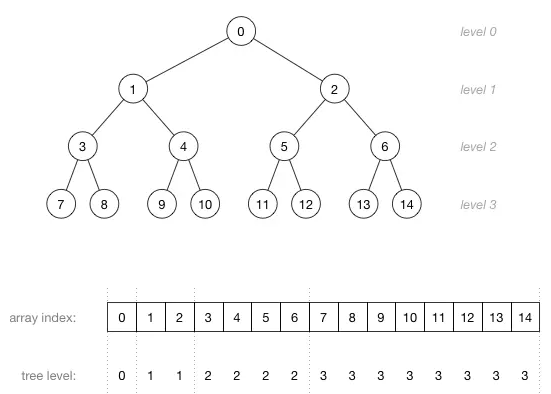
\includegraphics[scale=0.6]{20.png}
\end{center}

\subsection{二叉搜索树与堆的区别}

a. 在二叉搜索树中,左孩子一定比父节点小,右孩子一定比父节点大。而堆中要求孩子一定大于/小于父节点。

b. 因为堆仅用数组来存储数据,因此占用内存较小。

c. 二叉搜索树只有当“平衡”时,时间复杂度才能达到O(log(n));而堆直接能保证O(log(n))。

d. 搜索:二叉搜索树快,堆慢;插入/删除:堆快。


\subsection{构建堆}

\noindent 需要两个原始操作:

a. shiftUp(): 如果一个节点比它的\textbf{父}节点大(最大堆)或者小(最小堆),那么交换两节点。

b. shiftDown(): 如果一个节点比它的\textbf{子}节点小(最大堆)或者大(最小堆),那么交换两节点。该过程叫做“堆化heapify”。

\noindent 这两个操作是一个递归的过程,因此时间复杂度是O(log(n))

\noindent 其他操作:

insert(value)插入:在堆的尾部添加元素,并用shiftUp()来移动。

remove(root)移除根节点:将根结点直接删除,然后将堆尾元素移动至堆开头,然后用shiftUp(最小堆)/shiftDown(最大堆)来修复。

removeAtIndex(index)移除任意节点:将要删除的节点与堆尾节点交换位置,然后删除当前位于堆尾的要删除的节点。对刚刚交换上去的节点,根据情况进行修复操作。

\section{Dijkstra算法,最短路径,Prim/Kruskal算法,最小生成树}

\subsection{Dijkstras,最短路径}

\subsubsection{定义及例子} 该算法就是求两个节点的最短路径的。利用BFS思想(类似动态规划,即上一个结果对下一个运算有影响),直到目标点为止。适用于有向图和无向图。不能有边权为负的情况。
输出为:最短路径树。

\noindent 如图,有带权有向图,求s至每个结点的最短路径:

\begin{center}
    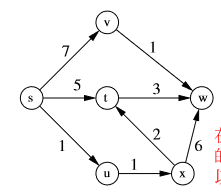
\includegraphics[scale=0.6]{21.png}\qquad
    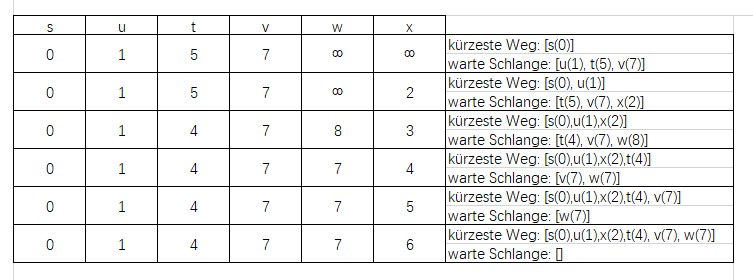
\includegraphics[scale=0.6]{22.png}
\end{center}

\subsubsection{算法} 

a. 建立两个队列,kürzeste Weg存储最短路径,warte Schlange存放刚被发现的节点至源点的距离。

b. 初始最短路径列表,将起始点放入

c. 选取等待队列中,路径长度最小的节点$x$:
    
\indent\indent i. 将$x$放入最短路径列表中(将最短路径存入最短路径列表中); 

\indent\indent ii. 在图中寻找与$x$直接相连的节点$m_i$,计算$wS(m_i) = w(x,m_i)+wS(x)$,并将结果放入warte Schlange列表中;

d. 重复c,直至warte Schlange列表为空。计算完成。

\subsubsection{带负权重的情况}

原始的dijkstra算法是不允许修改kürzeste Weg列表中的元素的,因此若图是带负权的,可能会找不到正确的最短路径。

因此,想要得到正确的结果,必须允许修改kW列表。

此外,不能通过“在所有的边上加上(-x)”来解决,得到的结果很有可能是错误的。因为,在$(s,...,m)$中,所经过的边越多,其路径长度变化越大,这无法保证每个最短路径是“公平”变化的。

\subsection{Prim算法(带Heap)}

\subsubsection{定义}

在加权连通图中,搜索最小生成树。

即,生成树中所有边权重之和最小。

\subsubsection{算法} 

\noindent 是基于动态规划的。

a. 从某一点$s$开始,寻找当前该点可以访问的所有的边$\{m_i\}$;

b. 在$\{m_i\}$中,选择最小边,判断该最小边的另一端是否访问过:

\indent\indent i. 若是,则跳过该边;

\indent\indent i. 若不是,则记录该边,并将另一端加入已访问节点集合中。

c. 重复b. 直至没有新的节点可以加入;

d. 此时,获得的树就是最小生成树。

\subsubsection{例子}

\noindent 求下图最小生成树

\begin{center}
    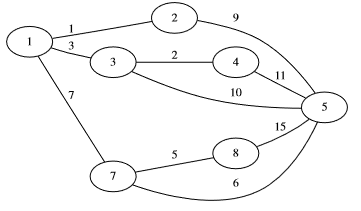
\includegraphics[scale=0.6]{23.png}\qquad
    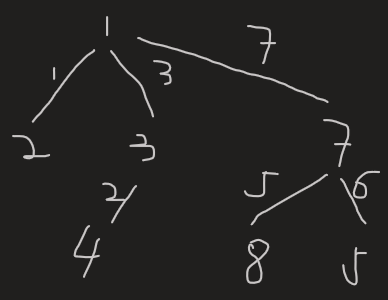
\includegraphics[scale=0.4]{24.png}
\end{center}

\subsection{Kruskal算法}

\subsubsection{定义}

也是用于寻找最小生成树,只不过,该算法更注重于边的关系。是基于贪心策略的。

\subsubsection{算法}

a. 将所有的边按照权重排序;

b. 选择权重最小的边,判断:若将该边加入已选择的边的集合后,是否生成了环:

\indent\indent i. 若有环,则放弃该边,继续;

\indent\indent i. 若没有环,则将该边加入其中。

c. 重复b. 直至有“节点总数-1”条边在集合之中。该集合就是生成树。

对于7.2.3的左图,按照kurskal算法,则步骤是:

选择边:(1,2), (3,4), (1,3), (7,8), (5,7), (1,7)。最终的生成树相同。

\section{最短路径,Floyd Warshall算法}

\subsection{定义}

用于寻找任意两点之间最短路径的算法。

可以正确处理有向图、带负权的图。

也可用于计算有向图的传递闭包。

\subsection{算法}

利用动态规划的思想,重新审视问题:

从任意节点$i$到任意节点$j$,不外乎2种可能:(1).直接从i到j;(2).i经过若干个节点到j。
因此:

a. 我们假设dis(i,j)为节点i,j的最短路径的距离,

b. 那么,对于每一个节点k,我们检查$dis(i,k)+dis(k,j) < dis(i,j)$是否成立:

\indent\indent i. 成立。则证明$i\rightarrow k \rightarrow j$路径长度比$i\rightarrow j$短,这时,我们设置$dis(i,j) = dis(i,k) + dis(k,j)$。

\indent\indent ii. 不成立,则continue;

c. 当遍历完所有的节点$k$,$dis(i,j)$记录的就是最短路径长度。

\subsection{具体计算:十字交叉法}

\begin{center}
    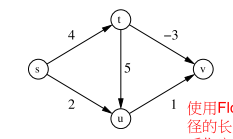
\includegraphics[scale=0.6]{25.png}
\end{center}

a. 先建立两个矩阵:

邻接矩阵$A_{-1}=\begin{pmatrix}
    0&4&2&\infty\\
    \infty&0&5&-3\\
    \infty&\infty&0&1\\
    \infty&\infty&\infty&0
\end{pmatrix}$
和用于记录中转节点的矩阵$Path_{-1}=\begin{pmatrix}
    -1&-1&-1&-1\\
    -1&-1&-1&-1\\
    -1&-1&-1&-1\\
    -1&-1&-1&-1\\
\end{pmatrix}$

b. 明确不能中转的状况:

\indent\indent i. $(u \rightarrow u)$不存在这种单点循环,因此[i][j]中,i==j的情况continue;

\indent\indent ii. $(i \rightarrow i \rightarrow j)$或$(i \rightarrow j \rightarrow j)$这种情况没有意义,因此$k == i$或$k==j$的情况continue;

c. 进入比较阶段,若$A[i][k] + A[k][j]<A[i][j]$:

\indent\indent i. 成立。则将$A[i][j] = A[i][k] + A[k][j]$,$Path[i][j] = k$

\indent\indent i. 不成立。continue;

d. 循环结束后,就可以通过$Path$矩阵找到任意两点的最短路径了。

\noindent b/c代码如下:

\begin{lstlisting}
for(int i = 0; i < 4; i++){
    for(int j =0; j < 4; j++){
        if(i == j){
            continue;
        }
        for(int k = 0; k < 4; k++){
            if(k == i || k == j){
                continue;
            }
            if(A[i][j]>A[i][k] + A[k][j]){
                A[i][j] = A[i][k] + A[k][j];
                Path[i][j] = k;
            }
        }
    }
}
\end{lstlisting}

\noindent d代码如下:

\begin{lstlisting}
Stack<Integer> t = new Stack<Integer>();
    
int u = i, v=j;
while (true) {
    t.push(v);
    if (this.Path[u][v] == -1) {
        break;
    }
    v = Path[u][v];
}
t.push(u);
\end{lstlisting}

\noindent 即,假设要找$(i,j)$之间的最短路径,那么:

a. 建立一个栈t,用于存储路径

b. 将j的值赋给v,将i的值赋给u;

c. 将v入栈,判断Path[i][j]的值是否是-1:

\indent\indent i. 若是:则中断循环;

\indent\indent i. 若不是:则将Path[u][v]的值赋给v;

d. 循环c. ,若循环终止,则表明已经找到最短路径,已经存在t中了。

e. 按顺序出栈,得到的序列就是最短路径。

\subsection{局限性}

当存在负权闭环时,该算法将找不到最短路径,很有可能陷入无限循环。形如下图。

\begin{center}
    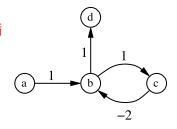
\includegraphics[scale=0.6]{26.png}
\end{center}

\section{最大流最小割,Ford-Fulkerson算法,Restnetzwerk}

\subsection{相关概念}

\noindent \textbf{Restnetzwerk残留网络:}

用途:让我们能够撤销上一个错误的决定(计算)。

为了能够撤销(undo)先前的流向决定,我们需要减小原先路径的可流量,并对应地增加反向路径的可流量。
因为:在残留网络中,反向路径的流量并不是说明我们真的可以倒着流,而是说明我们可以撤销先前在这条路径过来的“这么多”流量,并让它流向其他路径。

残余网络中的权重表示管道的空闲量,如下图初始化时:

\begin{center}
    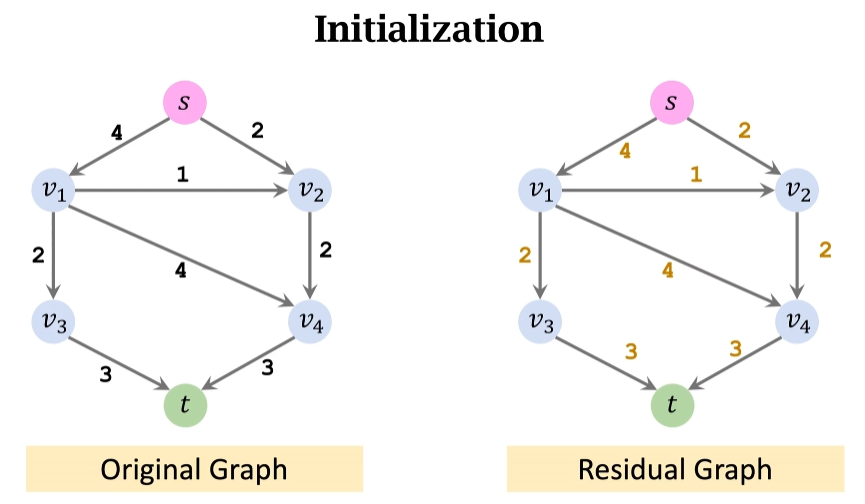
\includegraphics[scale=0.5]{27.png}
\end{center}

\subsection{Ford-Fulkerson算法}

重复以下步骤:

a. 在残余网络中寻找一条从出发点到目的地的可行路径,称为增广路径(argumenting path),若找不到,则结束循环;

b. 找出该路径中权值的最小值;

c. 用这一最小值更新路径中的前向边与反向边,当边为0是,拆边;

d. 将这一最小值累加到$max_flow$上($max_flow$初值为0)

最终得到的$max_flow$就是最大流。

其中,在a.中寻找增广路径的方法,可用DFS或BFS。若采用BFS,则称为Edmonds-Karp算法,该算法优于用DFS。

\noindent 例子:

第一轮迭代,找到的路径为$s-v_1-v_4-t$,路径最小值为3,那么修改残余网络如下左图。
可以看见,$v_4-t$这条边已经饱和了,这时,把它从残余网络中删除掉。

然后构建反向路径,提供“撤销操作”,如右图

\begin{center}
    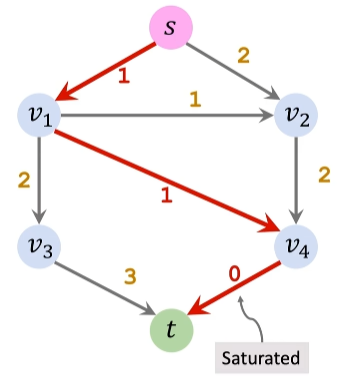
\includegraphics[scale=0.5]{28.png}
    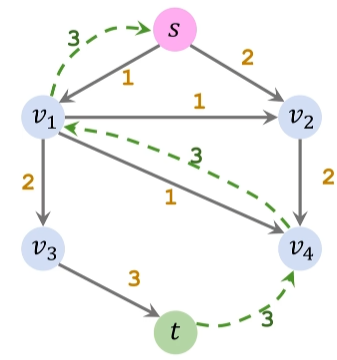
\includegraphics[scale=0.5]{29.png}
\end{center}

第二轮迭代:$s-v_1-v_3-t$。最小流量为1,因此将路径上的管道可用量-1,且$s-v_1$路径饱和了,这时删除该路径,得到如左图。

然后,构建反向路径,如右图

\begin{center}
    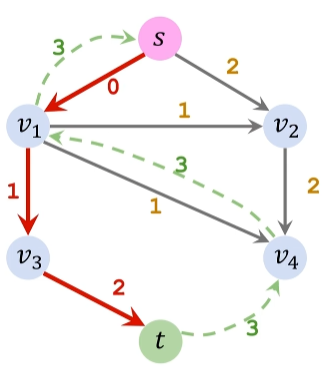
\includegraphics[scale=0.5]{30.png}
    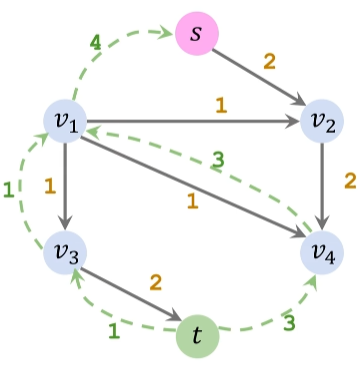
\includegraphics[scale=0.5]{31.png}
\end{center}

第三轮迭代:$s-v_2-v_4-v_1-v_3-t$,最小权重等于1,那么,将各个管道的空闲量-1,其中$v_1-v_3$饱和了,删去,得到如左图。

构建反向路径,如右图

\begin{center}
    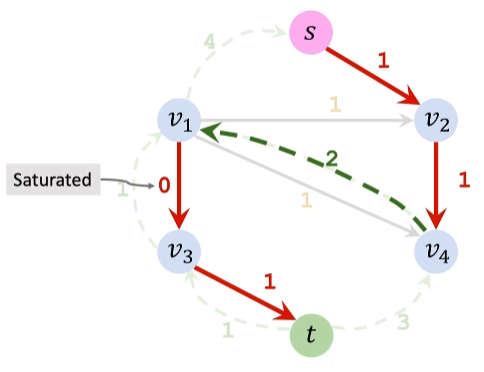
\includegraphics[scale=0.5]{32.png}
    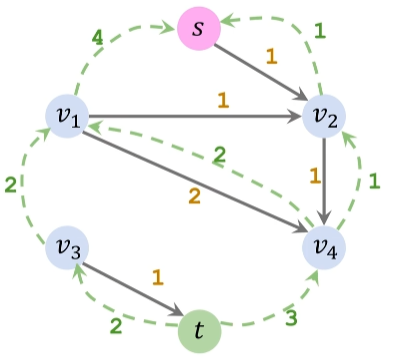
\includegraphics[scale=0.5]{33.png}
\end{center}

第四轮迭代:已经无法找到路径了,终止循环。将上右图与原图对比,可得下图。

数字左侧为流量$flow = capacity-residual$,即用原图上的数字减去上右图(残余网络图)中绿色的边上的值,不存在则为0。

总流量/最大流等于s的出流。

\begin{center}
    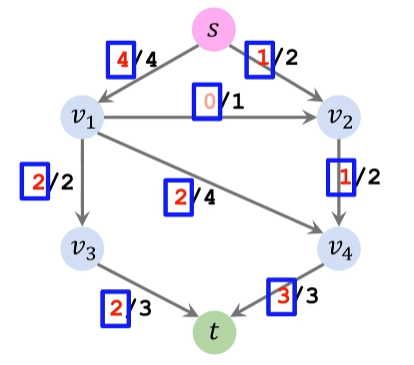
\includegraphics[scale=0.5]{34.png}
\end{center}

\section{最大二分匹配}

\subsection{定义:}

\noindent (1) 一个匹配:给定一个无向图$G=(V,E)$。其中,一个匹配指:$E$的某个子集$M$,对于所有的的节点$v\in V$,子集$M$中最多有一条边与$v$相连,那么称$v$由$M$匹配;否则就是没有匹配。

\noindent (2) 最大匹配:对于所有任意匹配$M'$,有$|M|\geq|M'|$的匹配$M$。

\noindent (3) 完美匹配:如果一个图的某个匹配中,所有的顶点都是匹配点,那么就是完美匹配。完美匹配一定是最大匹配。但最大匹配不一定是完美匹配。
\\
\\
人话:最大匹配就是求二分图中,两个集合中的顶点能成多少对。如果所有的点都用上了,就是完美匹配。

\subsection{用Ford-Fulkson解决最大二分匹配}

有以下一个二分图(左图,忽略颜色):

\begin{center}
    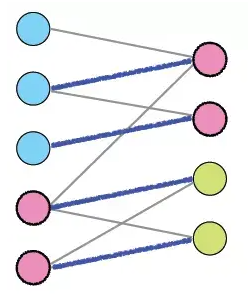
\includegraphics[scale=0.5]{35.png}
    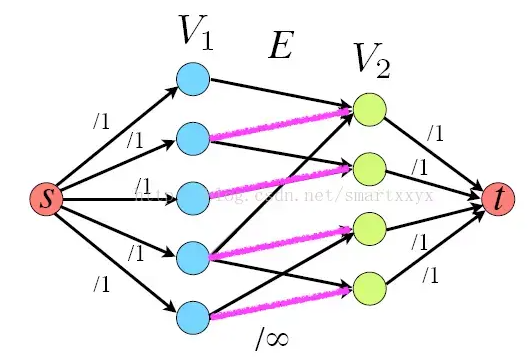
\includegraphics[scale=0.5]{36.png}
\end{center}

a. 把已有的边设为单向边($L\rightarrow R$),且各个边的容量均为$\infty$;

b. 增加源节点s和汇点t。将s与集合L中的节点相连,构造单向边$(s,l_i)$,设置容量为1。同理,设置$(r_i,t)$,容量为1。

c. 此时,得到了网络$G'$,该网络的最大流就等于最大匹配数。(上右图)

\section{动态规划}

\subsection{längste gemeinsame Teilfolge 最长公共子序列}

如有序列$A=cdbaeg,B=abdgae$,那么可以存在例如公共子序列$bae$。我们要找的是其中最长的。

\begin{center}
    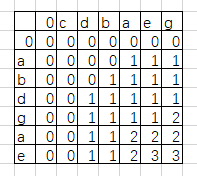
\includegraphics[scale=0.6]{37.png}
\end{center}

如上图,是规划完成的,最终右下角给的数值3,就是最长公共子序列长度。序列为最后一行数字变化的方格指向的字符,即"bae"。

\subsection{kürzeste gemeinsame Oberfolgen 最短公共超序列}

有字符串$A=abec,B=dbc$,则有其2个最短公共超序列$C_1=adbec,C_2=dabec$。

\subsubsection{方法1:利用LCS找SCS}

\begin{center}
    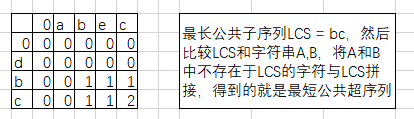
\includegraphics[scale=0.6]{38.png}
\end{center}

拼接规则:与$A,B$比较,将位于LCS中某个字符$lcs_i$之前(后)的字符,放到$lcs_i$之前(后)。

\subsubsection{方法2:用类似找LCS的思想,反推SCS}

\begin{center}
    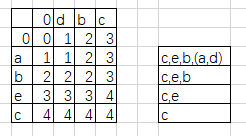
\includegraphics[scale=0.6]{39.png}
\end{center}

行为b{0,B},列为a{0,A},整个二维数组为scs[i][j]

\noindent 分两步

(a) 填表,第0行/列填入从0开始的递增序列,然后,对于scs[i][j]:

\indent\indent 若a[i]==b[j],则scs[i][j]=scs[i-1][j-1]+1;

\indent\indent 若a[i]!=b[j],则scs[i][j]=max(scs[i-1][j],scs[i][j-1]);

(b) 填好表之后,需要栈s。反向直接得出SCS串,对于scs[i][j]:

\indent\indent 若a[i]==b[j],则将scs[i][j]入栈s,然后i--,j--;

\indent\indent 若a[i]!=b[j],则比较scs[i-1][j],scs[i][j-1]:将大的一侧对应的字符入栈s,然后向小的一侧移动;若相等,则两个都入栈,顺序无所谓,然后向左上方移动;

当(b)循环结束后,最终可以得到栈s,按顺序出栈,就可以得到SCS串了。

\subsection{DP求最短路径}

\begin{center}
    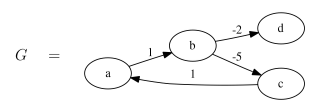
\includegraphics[scale=0.6]{40.png}
\end{center}

第8块的Floyed Warshall其实也是动态规划的,正好能解决这个问题。

\section{最优静态(二叉)搜索 optimalen statischen (Binär-) Suchbaum}

\subsection{定义}

\noindent \textbf{最优二叉搜索树:}给定n个不同的关键字组成的序列$K=<k_1,k_2...k_n>$,且关键字有序,如$(k_1<k_2<...<k_n)$,然后,我们要通过这些关键字,构造一颗二叉查找树。

对于每个关键字$k_i$,一次搜索能搜索到的概率为$p_i$。
\\
\\
\indent 假设要搜索$d$是否在$K$中,而$d$实际上并不存在于$K$,即$d\notin K$,这时,就需要设置$n+1$个虚拟键$(d_0,d_1...d_n)$,其代表不存在于$K$中的值,关系是:$(d_0<k_1<d_1<k_2<...<k_n<d_n)$。
\\
\\
\indent 而对于每个虚拟键,一次搜索能搜索到虚拟键的概率为$q_i$。
\\
\\
\indent 那么,为了使得超找一个节点的期望代价(比如从根结点到目标节点的路径上节点的数目)最小(即最快),就需要建立一颗最优二叉树。

\subsection{例子}

\subsubsection{暴力计算}

已知关键字和虚拟键的概率,求最优二叉搜索树:

\begin{center}
    \begin{tabular}{|c|c|c|c|c|c|c|}
        \hline
        $i$&0&1&2&3&4&5\\
        \hline
        $p_i$&&0.15&0.1&0.05&0.1&0.2\\
        \hline
        $q_i$&0.05&0.1&0.05&0.05&0.05&0.1\\
        \hline
    \end{tabular}
\end{center}

假设一次搜索的实际代价 = 检查的结点的个数。即,所发现的节点的深度+1。那么,一次搜索的期望代价等式为:

\begin{equation}
    \begin{split}
        E[search\, cost\, in\, T]&=\sum^n_{i=1}(depth_T(k_i)+1)\times p_i + \sum^n_{i=0}(depth_T(d_i)+1)\times q_i\\
        &=1+\sum^n_{i=1}(depth_T(k_i))\times p_i + \sum^n_{i=0}(depth_T(d_i))\times q_i
    \end{split}
\end{equation}

其中$\sum^n_{i=1}p_i+\sum^n_{i=0}q_i=1$。(实际上这就是个二项分布)

那么,根据上式,在要求上式结果最小的前提下,得到的二叉查找树,就是最优二叉查找树。
\\
\\
\indent 然而,在PDF中给出的情况,让我们无需考虑$q_i$的情况,因此,我们只考虑$p_i$。
那么:

$$K(T):=\sum^n_{i=1}p_i(Tiefe_T(a_i)+1)$$

具体操作上,就是,先把节点先随便组成一颗树,然后计算该树的Kost,选最小的就行了。

给出一个简单的例子:有$a,b,c$3点,概率分别是$\frac{5}{9},\frac{2}{9},\frac{2}{9}$。

(注:若$a,b,c$应有数学(大小)关系,构建的树为搜索二叉树。)

画出所有可能的搜索二叉树,分别计算Kost。

\begin{center}
    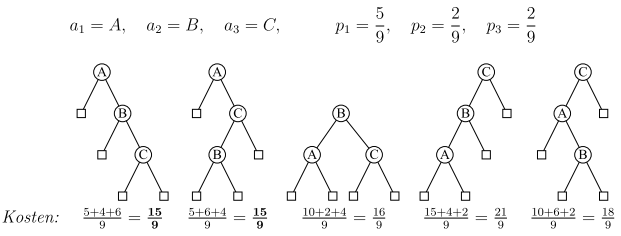
\includegraphics[scale=0.6]{41.png}
\end{center}

\subsubsection{递归计算,动态规划}

有数据如下表

\begin{center}
    \begin{tabular}{|c|c|c|c|c|}
        \hline
            Data&a&b&c&d\\
            \hline
            $p_i$&0.3&0.4&0.1&0.2\\
            \hline
    \end{tabular}
\end{center}

需要引入一个表T,用于存储子树期望,引入一个表K,用于记录父节点。对角线上的值即为单个节点的概率。第一行最后一个数据,为最终数据,即整棵树的最小期望。

$$T[h,k]=\sum^{k-h}_{i=k}p_i+min\{ \{T[k+1,h]\} \cup \{T[k,h-1]\} \cup \{T[k,i-1]+T[i+1,h]|k+1\leq i \leq h-1\} \}$$

利用上述公式,可得下左图。
\\
\\
\indent (e.g 1) 以$T[1,2]$为例,$T[1,2]=p_1+p_2+min\{T[1,1],T[2,2]\}$,其中$T[1,1]=0.3$比较小,所以被选中。这意味着在子树$T[1,2]$中,存在着更小的子树$T[1,1]$,并且在点$\{1,2\}$的关系中,2为1的父节点。因此,可以将2填入下中图中。
\\
\\
\indent (e.g 2) 以$T[1,4]$为例,$T[1,4]=p_1+p_2+p_3+p_4+\{T[1,3],T[2,4],T[1,1]+T[3,4],T[1,2]+T[4,4]\}$。其中,$T[1,1]+T[3,4]$最小,这意味着该树存在两个子树,分别是$T[1,1]$和$T[3,4]$,那么,不在子树上的节点就是父节点,也就是2。并且,此时已经可以得到整颗最优静态搜索树了:

\indent\indent 已知父节点为2,将2设置为根结点。已知存在两个子树$T[1,1]$和$T[3,4]$:

\indent\indent i. 其中$T[1,1]$表示单独的节点$a$,将其直接加入树中;

\indent\indent ii. $T[3,4]$表示一棵子树,查表K,可知该树的根结点为4。在之前计算$T[3,4]$的值的时候,应当同时记录了其子树,也就是$T[3,3]$,所以让3成为4的子节点。

至此,最优静态搜索树建立完毕如右图。


\begin{center}
    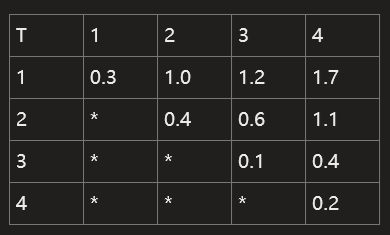
\includegraphics[scale=0.4]{42.png}
    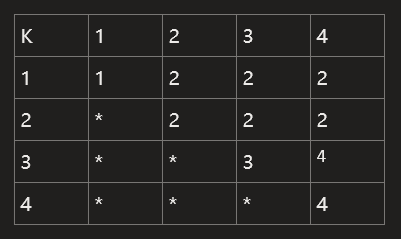
\includegraphics[scale=0.4]{43.png}
    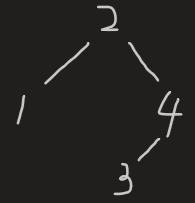
\includegraphics[scale=0.4]{44.png}
\end{center}











\section{Karazuba, 3-KNF, Davis-Putnam-Algorithmus}

\subsection{Karazuba}

\noindent 计算1100$\times$1011

\begin{tabular}{lr}
    &1100\\
    *&1011\\
    \hline\\
    &1100\\
    &1100 \ \! \\
    &0000 \ \! \ \! \\
    +&1100 \ \! \ \! \ \! \\
    \hline\\
    &10000100
\end{tabular}

gebrauchte Anzahl von Bit = 16 Bitmultiplikationen
\\
\\
Karazuba:

\begin{equation}
    \left\{
        \begin{array}{lr}
            1100 = x = x_h\cdot 2^{\frac{n}{2}} + x_l = 11\cdot 2^2 + 00\\
            1011 = y = y_h\cdot 2^{\frac{n}{2}} +y_l = 10\cdot 2^2 +11\\
            n = 4 \\
            P = (x_h + x_l)(y_h + y_l)
        \end{array}
    \right.
\end{equation}

$\Rightarrow x \cdot y = x_hy_h2^n+(P-x_hy_h-x_ly_l)2^{\frac{n}{2}} +x_ly_l$


\begin{equation}
    \begin{split}
        1100\times 1011 & = 11\times 10\times 2^4 + ((11+00)(10+11)-11\times 10 - 00\times 11)2^2+00\times 11 \\
        & = (1 \times 1 \times 2^2 + (10\times 1 - 1\times 1 - 1\times 0)2^1 + 0\times 1)2^4+(11\times 101 - 11\times 10)2^2 \\
        & = (100+(10-1)2^1)2^4 +(11\times 101 - 110)2^2 \\ 
        & = 110\times 2^4 + (1\times 10\times 2^2 + ((1+1)(10+1)-1\times 10 - 1\times 1)2^1 + 1\times 1 - 110)2^2\\
        & = 110\times 2^4 +1001\times 2^2\\
        & = 1000 \ 0100
    \end{split}
\end{equation}

gebrauchte Anzahl von Bit = 9 Bitmultiplikationen

\subsection{3-KNF, Davis-Putnam-Algorithmus}

已知逻辑运算F,要求用DPA进行化简,判断是否符合。

$F = (\neg A \vee B \vee C) \wedge (A \vee B \vee C) \wedge (A \vee B \vee \neg C)$

A = 0
\begin{equation}
\begin{split}
    & \ \ \ \ (1 \vee B \vee C) \wedge (0 \vee B \vee C) \wedge (0\vee B \vee \neg C)\\
    &= (B\vee C)\wedge (B\vee \neg C)
\end{split}
\end{equation}

B = 0

$\ \ \ \  = C \wedge \neg C$

B = 1

$ \ \ \ \ = (1\vee C)\wedge (1\vee \neg C)$

$ \ \ \ \ = 1$

return erfüllbar
\\
\\
\indent 或者如下图,先给B设置为0或1,然后依次推导。最终得到5个结果(Belegungen),其中有意义的为:

(1) 当B=1时,A/C任意;

(2) 当B=0, A=1时,C=1


\begin{center}
    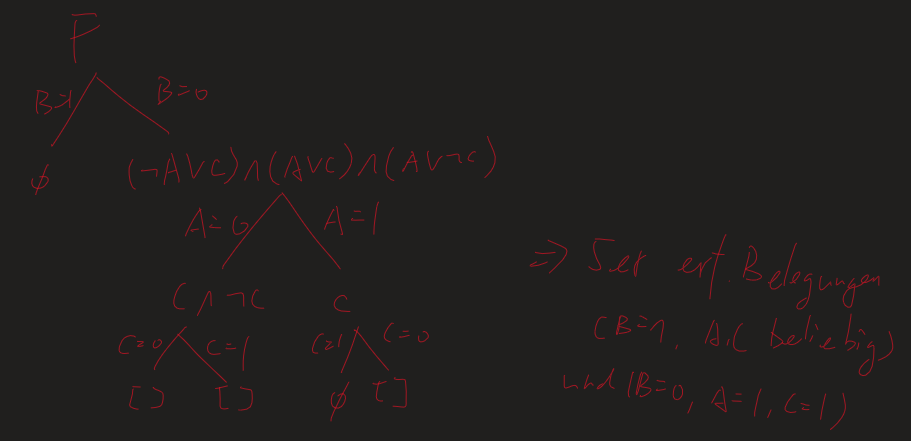
\includegraphics[scale=0.5]{45.png}
\end{center}





























































\end{document}